% =====================================================================
%  N6: tracking physical change, and flagging it early.
%
%  Upper panel reproduces the SETUP of the published drift experiment
%  (Shakouri, Kiriazes & Massoudieh 2026): Ksat,eng held at 10 m/day,
%  ramped to 2 m/day over one month, held at 2 thereafter, with the
%  assimilation's per-cycle estimate following it.
%  Lower panel is a SCHEMATIC of the CUSUM detector's behaviour.
%  Both curves are drawn, not exported from a run: the shape is the point.
%
%  Build: pdflatex fig_drift.tex && cp fig_drift.pdf figures/N6_drift_detection.pdf
% =====================================================================
\documentclass[border=4pt]{standalone}
\usepackage[T1]{fontenc}
\usepackage{helvet}
\renewcommand\familydefault{\sfdefault}
\usepackage{tikz}
\usepackage{pgfplots}
\pgfplotsset{compat=1.18}
\usetikzlibrary{arrows.meta,positioning,calc}

\definecolor{ohqblue}{HTML}{1F5C8B}
\definecolor{ohqteal}{HTML}{2A9D8F}
\definecolor{ohqrust}{HTML}{E76F51}
\definecolor{ohqgrey}{HTML}{6B7280}

\begin{document}
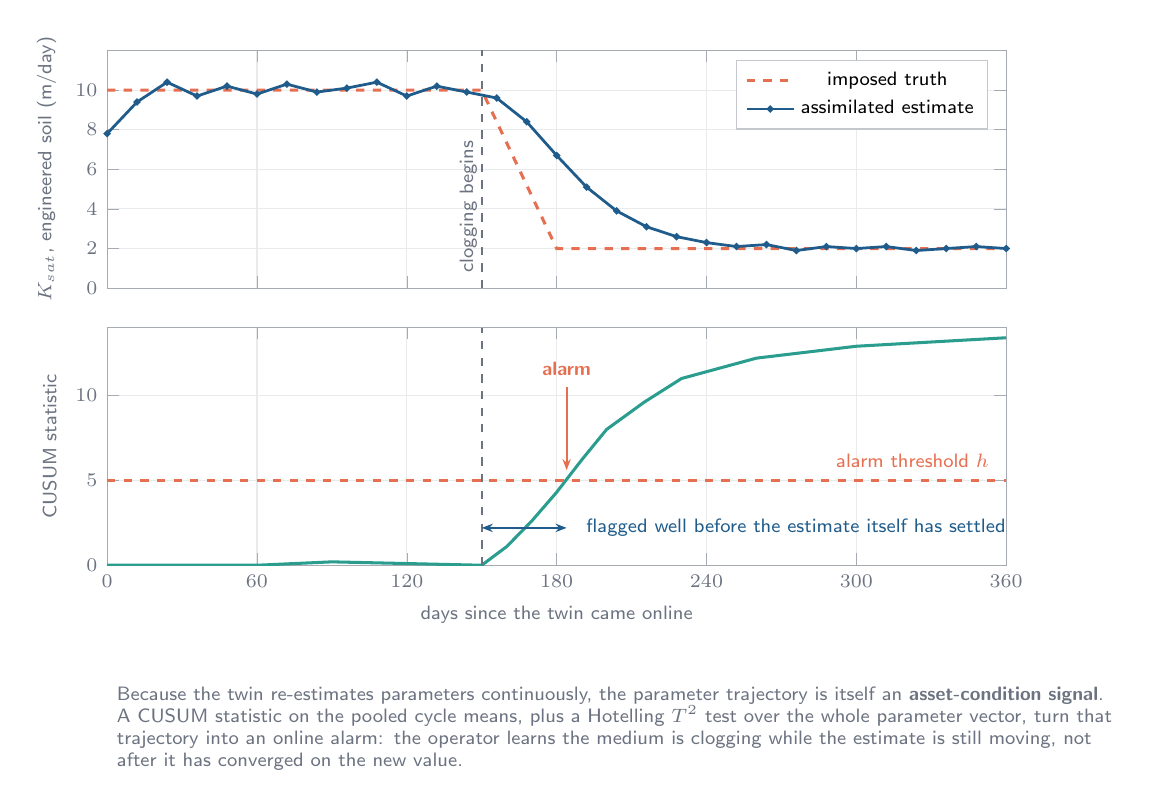
\begin{tikzpicture}[font=\sffamily]

\pgfplotsset{
  every axis/.append style={
    width=13cm, height=4.6cm,
    axis line style={ohqgrey!60}, tick style={ohqgrey!60},
    label style={font=\scriptsize, text=ohqgrey},
    tick label style={font=\scriptsize, text=ohqgrey},
    grid=major, major grid style={ohqgrey!15},
    xmin=0, xmax=360,
  },
}

% ---------------- upper: the parameter follows the change -----------
\begin{axis}[
  name=top,
  ylabel={$K_{sat}$, engineered soil (m/day)},
  ymin=0, ymax=12, ytick={0,2,4,6,8,10},
  xtick={0,60,120,180,240,300,360}, xticklabels={},
  legend style={font=\scriptsize, draw=ohqgrey!40, at={(0.98,0.96)},
                anchor=north east, fill=white},
]
% imposed truth: 10 until day 150, ramp to 2 by day 180, then 2
\addplot[ohqrust, line width=1.1pt, dashed] coordinates {
  (0,10) (150,10) (180,2) (360,2)};
\addlegendentry{imposed truth}
% the estimate: noisy, lags the ramp, settles on the new value
\addplot[ohqblue, line width=1pt, mark=*, mark size=0.7pt] coordinates {
  (0,7.8) (12,9.4) (24,10.4) (36,9.7) (48,10.2) (60,9.8) (72,10.3)
  (84,9.9) (96,10.1) (108,10.4) (120,9.7) (132,10.2) (144,9.9)
  (156,9.6) (168,8.4) (180,6.7) (192,5.1) (204,3.9) (216,3.1)
  (228,2.6) (240,2.3) (252,2.1) (264,2.2) (276,1.9) (288,2.1)
  (300,2.0) (312,2.1) (324,1.9) (336,2.0) (348,2.1) (360,2.0)};
\addlegendentry{assimilated estimate}
\draw[ohqgrey, dashed, line width=0.7pt] (axis cs:150,0) -- (axis cs:150,12);
\node[font=\scriptsize, text=ohqgrey, anchor=south west, rotate=90]
  at (axis cs:152,0.3) {clogging begins};
\end{axis}

% ---------------- lower: the detector fires first -------------------
\begin{axis}[
  name=bot, at={(top.below south west)}, anchor=north west, yshift=-6pt,
  xlabel={days since the twin came online},
  ylabel={CUSUM statistic},
  ymin=0, ymax=14, ytick={0,5,10},
  xtick={0,60,120,180,240,300,360},
]
\addplot[ohqteal, line width=1.1pt] coordinates {
  (0,0) (30,0) (60,0) (90,0.2) (120,0.1) (150,0) (160,1.1) (170,2.6)
  (180,4.3) (190,6.2) (200,8.0) (215,9.6) (230,11.0) (260,12.2)
  (300,12.9) (360,13.4)};
\draw[ohqrust, line width=0.9pt, dashed]
  (axis cs:0,5) -- (axis cs:360,5);
\node[font=\scriptsize, text=ohqrust, anchor=south east]
  at (axis cs:357,5.2) {alarm threshold $h$};
\draw[ohqgrey, dashed, line width=0.7pt] (axis cs:150,0) -- (axis cs:150,14);
\draw[ohqrust, line width=0.7pt, -{Stealth[length=4pt]}]
  (axis cs:184,10.5) -- (axis cs:184,5.6);
\node[font=\scriptsize\bfseries, text=ohqrust, anchor=south]
  at (axis cs:184,10.6) {alarm};
\draw[{Stealth[length=4pt]}-{Stealth[length=4pt]}, ohqblue, line width=0.7pt]
  (axis cs:150,2.2) -- (axis cs:184,2.2);
\node[font=\scriptsize, text=ohqblue, anchor=west] at (axis cs:188,2.2)
  {flagged well before the estimate itself has settled};
\end{axis}

\node[font=\scriptsize, text=ohqgrey, anchor=north west, text width=128mm,
      align=left] at ($(bot.below south west)+(0,-16pt)$)
  {Because the twin re-estimates parameters continuously, the parameter
   trajectory is itself an \textbf{asset-condition signal}. A CUSUM statistic
   on the pooled cycle means, plus a Hotelling $T^2$ test over the whole
   parameter vector, turn that trajectory into an online alarm: the operator
   learns the medium is clogging while the estimate is still moving, not after
   it has converged on the new value.};

\end{tikzpicture}
\end{document}
